\documentclass[tikz]{standalone}

\definecolor{n0}{HTML}{785EF0}
\definecolor{End}{HTML}{DC267F}
\definecolor{Corner}{HTML}{FFB000}
\definecolor{NewHex}{HTML}{648FFF}
\definecolor{Reversal}{HTML}{FE6100}

\begin{document}
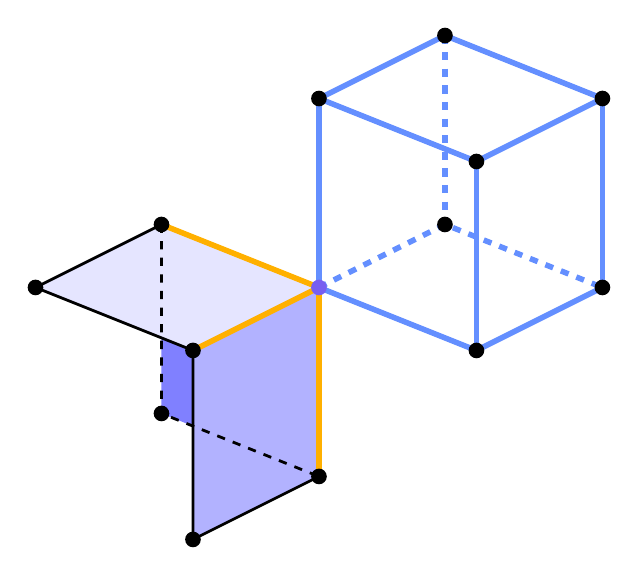
\begin{tikzpicture}[scale=4, x={(0.5cm,-0.2cm)}, y={(0.4cm,0.2cm)}, z={(0.0cm,0.6cm)}]

  %%%%%%%%%% Points pour travailler %%%%%%%%%%
  \coordinate (0) at (0,0,0);
  \coordinate (1) at (0,-1,-1);
  \coordinate (2) at (0,0,-1);
  \coordinate (3) at (-1,0,-1);
  \coordinate (4) at (0,-1,0);
  \coordinate (5) at (-1,-1,0);
  \coordinate (6) at (-1,0,0);
  \coordinate (7) at (0,0,1);
  \coordinate (8) at (0,1,1);
  \coordinate (9) at (1,1,1);
  \coordinate (10) at (1,0,1);
  \coordinate (11) at (0,1,0);
  \coordinate (12) at (1,1,0);
  \coordinate (13) at (1,0,0);
  
%%%%%%%%%% Layer blue color %%%%%%%%%%
\fill [color=blue!50!white] (0) -- (2) -- (3) -- (6) -- cycle ;
\fill [color=blue!30!white] (0) -- (2) -- (1) -- (4) -- cycle ;
\fill [color=blue!10!white] (0) -- (4) -- (5) -- (6) -- cycle ;

 %%%%%%%%%%%%%%%% Precedant layer %%%%%%%%%%%%%%%%%%%
\draw [line width=1] (6) -- (5) -- (4) -- (1) -- (2) ;
\draw [line width=1, dashed] (6) -- (3) -- (2) ;

 %%%%%%%%%%% Feature edges %%%%%%%%%%%
\draw [line width=2, color=Corner] (0) -- (6) ;
\draw [line width=2, color=Corner] (0) -- (4) ;
\draw [line width=2, color=Corner] (0) -- (2) ;

 %%%%%%%%%%% The HEXAS created %%%%%%%%%%% 
\draw [line width=2, color=NewHex] (0) -- (13) -- (12) ;
 \draw [line width=2, color=NewHex] (7) -- (8) -- (9) -- (10) -- (7) ;
 \draw [line width=2, color=NewHex] (0) -- (7) ;
 \draw [line width=2, color=NewHex] (13) -- (10) ;
 \draw [line width=2, color=NewHex] (12) -- (9) ;

 \draw [dashed, line width=2, color=NewHex] (0) -- (11) -- (12) ;
 \draw [dashed, line width=2, color=NewHex] (8) -- (11) ;

 %%%%%%%%%%% HEXA NODES %%%%%%%%%%%
  \foreach \i in {1,...,13}
 {
   \draw (\i) node[circle, fill=black, inner sep = 2 pt] {};
 }
 \draw (0) node[circle, fill=n0, inner sep = 2 pt] {};

\end{tikzpicture}
\end{document}